\documentclass[twoside]{book}

% Packages required by doxygen
\usepackage{fixltx2e}
\usepackage{calc}
\usepackage{doxygen}
\usepackage[export]{adjustbox} % also loads graphicx
\usepackage{graphicx}
\usepackage[utf8]{inputenc}
\usepackage{makeidx}
\usepackage{multicol}
\usepackage{multirow}
\PassOptionsToPackage{warn}{textcomp}
\usepackage{textcomp}
\usepackage[nointegrals]{wasysym}
\usepackage[table]{xcolor}

% Font selection
\usepackage[T1]{fontenc}
\usepackage[scaled=.90]{helvet}
\usepackage{courier}
\usepackage{amssymb}
\usepackage{sectsty}
\renewcommand{\familydefault}{\sfdefault}
\allsectionsfont{%
  \fontseries{bc}\selectfont%
  \color{darkgray}%
}
\renewcommand{\DoxyLabelFont}{%
  \fontseries{bc}\selectfont%
  \color{darkgray}%
}
\newcommand{\+}{\discretionary{\mbox{\scriptsize$\hookleftarrow$}}{}{}}

% Page & text layout
\usepackage{geometry}
\geometry{%
  a4paper,%
  top=2.5cm,%
  bottom=2.5cm,%
  left=2.5cm,%
  right=2.5cm%
}
\tolerance=750
\hfuzz=15pt
\hbadness=750
\setlength{\emergencystretch}{15pt}
\setlength{\parindent}{0cm}
\setlength{\parskip}{3ex plus 2ex minus 2ex}
\makeatletter
\renewcommand{\paragraph}{%
  \@startsection{paragraph}{4}{0ex}{-1.0ex}{1.0ex}{%
    \normalfont\normalsize\bfseries\SS@parafont%
  }%
}
\renewcommand{\subparagraph}{%
  \@startsection{subparagraph}{5}{0ex}{-1.0ex}{1.0ex}{%
    \normalfont\normalsize\bfseries\SS@subparafont%
  }%
}
\makeatother

% Headers & footers
\usepackage{fancyhdr}
\pagestyle{fancyplain}
\fancyhead[LE]{\fancyplain{}{\bfseries\thepage}}
\fancyhead[CE]{\fancyplain{}{}}
\fancyhead[RE]{\fancyplain{}{\bfseries\leftmark}}
\fancyhead[LO]{\fancyplain{}{\bfseries\rightmark}}
\fancyhead[CO]{\fancyplain{}{}}
\fancyhead[RO]{\fancyplain{}{\bfseries\thepage}}
\fancyfoot[LE]{\fancyplain{}{}}
\fancyfoot[CE]{\fancyplain{}{}}
\fancyfoot[RE]{\fancyplain{}{\bfseries\scriptsize Generated by Doxygen }}
\fancyfoot[LO]{\fancyplain{}{\bfseries\scriptsize Generated by Doxygen }}
\fancyfoot[CO]{\fancyplain{}{}}
\fancyfoot[RO]{\fancyplain{}{}}
\renewcommand{\footrulewidth}{0.4pt}
\renewcommand{\chaptermark}[1]{%
  \markboth{#1}{}%
}
\renewcommand{\sectionmark}[1]{%
  \markright{\thesection\ #1}%
}

% Indices & bibliography
\usepackage{natbib}
\usepackage[titles]{tocloft}
\setcounter{tocdepth}{3}
\setcounter{secnumdepth}{5}
\makeindex

% Hyperlinks (required, but should be loaded last)
\usepackage{ifpdf}
\ifpdf
  \usepackage[pdftex,pagebackref=true]{hyperref}
\else
  \usepackage[ps2pdf,pagebackref=true]{hyperref}
\fi
\hypersetup{%
  colorlinks=true,%
  linkcolor=blue,%
  citecolor=blue,%
  unicode%
}

% Custom commands
\newcommand{\clearemptydoublepage}{%
  \newpage{\pagestyle{empty}\cleardoublepage}%
}

\usepackage{caption}
\captionsetup{labelsep=space,justification=centering,font={bf},singlelinecheck=off,skip=4pt,position=top}

%===== C O N T E N T S =====

\begin{document}

% Titlepage & ToC
\hypersetup{pageanchor=false,
             bookmarksnumbered=true,
             pdfencoding=unicode
            }
\pagenumbering{alph}
\begin{titlepage}
\vspace*{7cm}
\begin{center}%
{\Large My Project }\\
\vspace*{1cm}
{\large Generated by Doxygen 1.8.13}\\
\end{center}
\end{titlepage}
\clearemptydoublepage
\pagenumbering{roman}
\tableofcontents
\clearemptydoublepage
\pagenumbering{arabic}
\hypersetup{pageanchor=true}

%--- Begin generated contents ---
\chapter{Class Index}
\section{Class List}
Here are the classes, structs, unions and interfaces with brief descriptions\+:\begin{DoxyCompactList}
\item\contentsline{section}{\hyperlink{structbackground}{background} }{\pageref{structbackground}}{}
\item\contentsline{section}{\hyperlink{structenigme}{enigme} }{\pageref{structenigme}}{}
\item\contentsline{section}{\hyperlink{structEnigmex}{Enigmex} }{\pageref{structEnigmex}}{}
\item\contentsline{section}{\hyperlink{structennemis}{ennemis} }{\pageref{structennemis}}{}
\item\contentsline{section}{\hyperlink{structennemyx}{ennemyx} }{\pageref{structennemyx}}{}
\item\contentsline{section}{\hyperlink{structfirex}{firex} }{\pageref{structfirex}}{}
\item\contentsline{section}{\hyperlink{structMenu}{Menu} }{\pageref{structMenu}}{}
\item\contentsline{section}{\hyperlink{structObjet}{Objet} }{\pageref{structObjet}}{}
\item\contentsline{section}{\hyperlink{structperso}{perso} }{\pageref{structperso}}{}
\item\contentsline{section}{\hyperlink{structsaves}{saves} }{\pageref{structsaves}}{}
\item\contentsline{section}{\hyperlink{structvie}{vie} }{\pageref{structvie}}{}
\end{DoxyCompactList}

\chapter{File Index}
\section{File List}
Here is a list of all documented files with brief descriptions\+:\begin{DoxyCompactList}
\item\contentsline{section}{{\bfseries arduino.\+h} }{\pageref{arduino_8h}}{}
\item\contentsline{section}{{\bfseries background.\+h} }{\pageref{background_8h}}{}
\item\contentsline{section}{{\bfseries collision.\+h} }{\pageref{collision_8h}}{}
\item\contentsline{section}{{\bfseries enig.\+h} }{\pageref{enig_8h}}{}
\item\contentsline{section}{{\bfseries enigmedyn.\+h} }{\pageref{enigmedyn_8h}}{}
\item\contentsline{section}{{\bfseries ennemi.\+h} }{\pageref{ennemi_8h}}{}
\item\contentsline{section}{{\bfseries fonction.\+h} }{\pageref{fonction_8h}}{}
\item\contentsline{section}{{\bfseries gamemenu.\+h} }{\pageref{gamemenu_8h}}{}
\item\contentsline{section}{{\bfseries ia.\+h} }{\pageref{ia_8h}}{}
\item\contentsline{section}{\hyperlink{main_8c}{main.\+c} \\*Testing program  ragnarok }{\pageref{main_8c}}{}
\item\contentsline{section}{{\bfseries Menu1.\+h} }{\pageref{Menu1_8h}}{}
\item\contentsline{section}{{\bfseries minimapfunc.\+h} }{\pageref{minimapfunc_8h}}{}
\item\contentsline{section}{{\bfseries object.\+h} }{\pageref{object_8h}}{}
\item\contentsline{section}{{\bfseries playermov.\+h} }{\pageref{playermov_8h}}{}
\item\contentsline{section}{{\bfseries rot.\+h} }{\pageref{rot_8h}}{}
\item\contentsline{section}{{\bfseries scrolling.\+h} }{\pageref{scrolling_8h}}{}
\item\contentsline{section}{{\bfseries utility.\+h} }{\pageref{utility_8h}}{}
\end{DoxyCompactList}

\chapter{Class Documentation}
\hypertarget{structbackground}{}\section{background Struct Reference}
\label{structbackground}\index{background@{background}}
\subsection*{Public Attributes}
\begin{DoxyCompactItemize}
\item 
\mbox{\Hypertarget{structbackground_a3f481de34cfa3f9538aa074589823614}\label{structbackground_a3f481de34cfa3f9538aa074589823614}} 
S\+D\+L\+\_\+\+Surface $\ast$ {\bfseries fond}
\item 
\mbox{\Hypertarget{structbackground_ad986c299e38f559476b1d5d3f1b4ea99}\label{structbackground_ad986c299e38f559476b1d5d3f1b4ea99}} 
Mix\+\_\+\+Music $\ast$ {\bfseries musique}
\item 
\mbox{\Hypertarget{structbackground_a7adc1acf00dd3f9425a98205a0ea9c0a}\label{structbackground_a7adc1acf00dd3f9425a98205a0ea9c0a}} 
S\+D\+L\+\_\+\+Rect {\bfseries position\+Fond}
\end{DoxyCompactItemize}


The documentation for this struct was generated from the following file\+:\begin{DoxyCompactItemize}
\item 
Menu1.\+h\end{DoxyCompactItemize}

\hypertarget{structenigme}{}\section{enigme Struct Reference}
\label{structenigme}\index{enigme@{enigme}}
\subsection*{Public Attributes}
\begin{DoxyCompactItemize}
\item 
\mbox{\Hypertarget{structenigme_aed2865ec5864f0d48865e23210a615e5}\label{structenigme_aed2865ec5864f0d48865e23210a615e5}} 
S\+D\+L\+\_\+\+Surface $\ast$ {\bfseries img}
\item 
\mbox{\Hypertarget{structenigme_a1ecc3fa572d2c308e1aecacf74fd1ec0}\label{structenigme_a1ecc3fa572d2c308e1aecacf74fd1ec0}} 
S\+D\+L\+\_\+\+Rect {\bfseries p}
\end{DoxyCompactItemize}


The documentation for this struct was generated from the following files\+:\begin{DoxyCompactItemize}
\item 
enig.\+h\item 
playermov.\+h\end{DoxyCompactItemize}

\hypertarget{structEnigmex}{}\section{Enigmex Struct Reference}
\label{structEnigmex}\index{Enigmex@{Enigmex}}
\subsection*{Public Attributes}
\begin{DoxyCompactItemize}
\item 
\mbox{\Hypertarget{structEnigmex_a8614f4b442356e05b40439cd99b6c264}\label{structEnigmex_a8614f4b442356e05b40439cd99b6c264}} 
S\+D\+L\+\_\+\+Rect {\bfseries tab} \mbox{[}4\mbox{]}\mbox{[}4\mbox{]}
\item 
\mbox{\Hypertarget{structEnigmex_a3d381a1d84fc00ab3e9edb2964b38af0}\label{structEnigmex_a3d381a1d84fc00ab3e9edb2964b38af0}} 
char {\bfseries nomimage} \mbox{[}30\mbox{]}
\end{DoxyCompactItemize}


The documentation for this struct was generated from the following files\+:\begin{DoxyCompactItemize}
\item 
enigmedyn.\+c\item 
enigmedyn.\+h\end{DoxyCompactItemize}

\hypertarget{structennemis}{}\section{ennemis Struct Reference}
\label{structennemis}\index{ennemis@{ennemis}}
\subsection*{Public Attributes}
\begin{DoxyCompactItemize}
\item 
\mbox{\Hypertarget{structennemis_a3e8a9864c41c217f29e8fa94c3323414}\label{structennemis_a3e8a9864c41c217f29e8fa94c3323414}} 
S\+D\+L\+\_\+\+Rect {\bfseries position}
\item 
\mbox{\Hypertarget{structennemis_a25ac4c539f00f1d72a98164bbbe17f18}\label{structennemis_a25ac4c539f00f1d72a98164bbbe17f18}} 
S\+D\+L\+\_\+\+Rect {\bfseries position2}
\item 
\mbox{\Hypertarget{structennemis_a12545f1dec3d4c2f47ea779e08a832bd}\label{structennemis_a12545f1dec3d4c2f47ea779e08a832bd}} 
S\+D\+L\+\_\+\+Surface $\ast$ {\bfseries fond}
\item 
\mbox{\Hypertarget{structennemis_ad566435b5e86ee846b20ca8c261a9d9f}\label{structennemis_ad566435b5e86ee846b20ca8c261a9d9f}} 
S\+D\+L\+\_\+\+Surface $\ast$ {\bfseries fond1}
\item 
\mbox{\Hypertarget{structennemis_a7cdce135302cefeedce69637c561ca87}\label{structennemis_a7cdce135302cefeedce69637c561ca87}} 
S\+D\+L\+\_\+\+Surface $\ast$ {\bfseries fond2}
\item 
\mbox{\Hypertarget{structennemis_a966a4674686ad60c8f77acf31d1f4a08}\label{structennemis_a966a4674686ad60c8f77acf31d1f4a08}} 
S\+D\+L\+\_\+\+Surface $\ast$ {\bfseries fond3}
\item 
\mbox{\Hypertarget{structennemis_a16abd6014e78ee7fdf5ab944bc2946a4}\label{structennemis_a16abd6014e78ee7fdf5ab944bc2946a4}} 
S\+D\+L\+\_\+\+Surface $\ast$ {\bfseries fond4}
\item 
\mbox{\Hypertarget{structennemis_a0656bf1f2a05bd147d373d7eaa3f4285}\label{structennemis_a0656bf1f2a05bd147d373d7eaa3f4285}} 
S\+D\+L\+\_\+\+Surface $\ast$ {\bfseries fonda}
\item 
\mbox{\Hypertarget{structennemis_aaef083b31ba478455bcbd16ed7235efb}\label{structennemis_aaef083b31ba478455bcbd16ed7235efb}} 
S\+D\+L\+\_\+\+Surface $\ast$ {\bfseries fondb}
\item 
\mbox{\Hypertarget{structennemis_abcddeea26249480501c3f691e5611345}\label{structennemis_abcddeea26249480501c3f691e5611345}} 
S\+D\+L\+\_\+\+Surface $\ast$ {\bfseries fondc}
\item 
\mbox{\Hypertarget{structennemis_ab982bb15caada636f5986421676d2183}\label{structennemis_ab982bb15caada636f5986421676d2183}} 
S\+D\+L\+\_\+\+Surface $\ast$ {\bfseries fondd}
\item 
\mbox{\Hypertarget{structennemis_ad44f2c7a54b691c3f3cc510256939700}\label{structennemis_ad44f2c7a54b691c3f3cc510256939700}} 
int {\bfseries active}
\item 
\mbox{\Hypertarget{structennemis_a346ebf1f4750af9f17b319c0866baf72}\label{structennemis_a346ebf1f4750af9f17b319c0866baf72}} 
int {\bfseries posmin}
\item 
\mbox{\Hypertarget{structennemis_a71ee9866c26653b85099cfb9052557db}\label{structennemis_a71ee9866c26653b85099cfb9052557db}} 
int {\bfseries posmax}
\item 
\mbox{\Hypertarget{structennemis_af075a9a9a64e296a56836d4dffda748f}\label{structennemis_af075a9a9a64e296a56836d4dffda748f}} 
int {\bfseries mvmspeed}
\item 
\mbox{\Hypertarget{structennemis_a713a84f00226c69f8b162ba2a4690c6f}\label{structennemis_a713a84f00226c69f8b162ba2a4690c6f}} 
int {\bfseries z}
\item 
\mbox{\Hypertarget{structennemis_a2dc78c4652791527589b6f4d30098075}\label{structennemis_a2dc78c4652791527589b6f4d30098075}} 
int {\bfseries x}
\end{DoxyCompactItemize}


The documentation for this struct was generated from the following file\+:\begin{DoxyCompactItemize}
\item 
ennemi.\+h\end{DoxyCompactItemize}

\hypertarget{structennemyx}{}\section{ennemyx Struct Reference}
\label{structennemyx}\index{ennemyx@{ennemyx}}
\subsection*{Public Attributes}
\begin{DoxyCompactItemize}
\item 
\mbox{\Hypertarget{structennemyx_ad2a12aa07cad08723a63574c1f2ebd07}\label{structennemyx_ad2a12aa07cad08723a63574c1f2ebd07}} 
S\+D\+L\+\_\+\+Surface $\ast$ {\bfseries right1}
\item 
\mbox{\Hypertarget{structennemyx_ace9895186ea99359152696520fa22247}\label{structennemyx_ace9895186ea99359152696520fa22247}} 
S\+D\+L\+\_\+\+Surface $\ast$ {\bfseries right2}
\item 
\mbox{\Hypertarget{structennemyx_ae9f0674de0f5b27b7c26ec7c9e5e2be4}\label{structennemyx_ae9f0674de0f5b27b7c26ec7c9e5e2be4}} 
S\+D\+L\+\_\+\+Surface $\ast$ {\bfseries right3}
\item 
\mbox{\Hypertarget{structennemyx_a22cf0fc6fefe2676dc0a14e18931f3bd}\label{structennemyx_a22cf0fc6fefe2676dc0a14e18931f3bd}} 
S\+D\+L\+\_\+\+Surface $\ast$ {\bfseries right4}
\item 
\mbox{\Hypertarget{structennemyx_a913b4f00a14d849e0369385ad162e88b}\label{structennemyx_a913b4f00a14d849e0369385ad162e88b}} 
S\+D\+L\+\_\+\+Surface $\ast$ {\bfseries left1}
\item 
\mbox{\Hypertarget{structennemyx_a49303d5596d7d0cf9d14338b83f755c0}\label{structennemyx_a49303d5596d7d0cf9d14338b83f755c0}} 
S\+D\+L\+\_\+\+Surface $\ast$ {\bfseries left2}
\item 
\mbox{\Hypertarget{structennemyx_ae414742c72e450d88af5f4af4782b687}\label{structennemyx_ae414742c72e450d88af5f4af4782b687}} 
S\+D\+L\+\_\+\+Surface $\ast$ {\bfseries left3}
\item 
\mbox{\Hypertarget{structennemyx_a07dc2a14cadfc08084accc4791b35354}\label{structennemyx_a07dc2a14cadfc08084accc4791b35354}} 
S\+D\+L\+\_\+\+Surface $\ast$ {\bfseries left4}
\end{DoxyCompactItemize}


The documentation for this struct was generated from the following file\+:\begin{DoxyCompactItemize}
\item 
ia.\+h\end{DoxyCompactItemize}

\hypertarget{structfirex}{}\section{firex Struct Reference}
\label{structfirex}\index{firex@{firex}}
\subsection*{Public Attributes}
\begin{DoxyCompactItemize}
\item 
\mbox{\Hypertarget{structfirex_a5c3030f2b859db89d4fd83458a4201f7}\label{structfirex_a5c3030f2b859db89d4fd83458a4201f7}} 
S\+D\+L\+\_\+\+Surface $\ast$ {\bfseries fire1}
\item 
\mbox{\Hypertarget{structfirex_ad0e98fd735fa54b004b726225d0d31c8}\label{structfirex_ad0e98fd735fa54b004b726225d0d31c8}} 
S\+D\+L\+\_\+\+Surface $\ast$ {\bfseries fire2}
\end{DoxyCompactItemize}


The documentation for this struct was generated from the following file\+:\begin{DoxyCompactItemize}
\item 
ia.\+h\end{DoxyCompactItemize}

\hypertarget{structMenu}{}\section{Menu Struct Reference}
\label{structMenu}\index{Menu@{Menu}}


Collaboration diagram for Menu\+:
\nopagebreak
\begin{figure}[H]
\begin{center}
\leavevmode
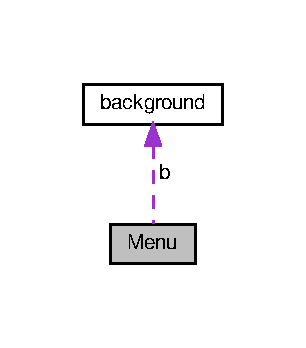
\includegraphics[width=147pt]{structMenu__coll__graph}
\end{center}
\end{figure}
\subsection*{Public Attributes}
\begin{DoxyCompactItemize}
\item 
\mbox{\Hypertarget{structMenu_ace635e2f2ed8aa326e894c8d879148d6}\label{structMenu_ace635e2f2ed8aa326e894c8d879148d6}} 
\hyperlink{structbackground}{background} {\bfseries b}
\item 
\mbox{\Hypertarget{structMenu_ae29eb7a1c451ac7d1977a09e0f0f8d65}\label{structMenu_ae29eb7a1c451ac7d1977a09e0f0f8d65}} 
Mix\+\_\+\+Music $\ast$ {\bfseries but}
\end{DoxyCompactItemize}


The documentation for this struct was generated from the following file\+:\begin{DoxyCompactItemize}
\item 
Menu1.\+h\end{DoxyCompactItemize}

\hypertarget{structObjet}{}\section{Objet Struct Reference}
\label{structObjet}\index{Objet@{Objet}}
\subsection*{Public Attributes}
\begin{DoxyCompactItemize}
\item 
\mbox{\Hypertarget{structObjet_adc26449d5051fc613b8972a08a3e7bba}\label{structObjet_adc26449d5051fc613b8972a08a3e7bba}} 
S\+D\+L\+\_\+\+Surface $\ast$ {\bfseries image}
\item 
\mbox{\Hypertarget{structObjet_a92fd979dc6d37621933bf051914da800}\label{structObjet_a92fd979dc6d37621933bf051914da800}} 
S\+D\+L\+\_\+\+Rect {\bfseries position}
\end{DoxyCompactItemize}


The documentation for this struct was generated from the following file\+:\begin{DoxyCompactItemize}
\item 
object.\+h\end{DoxyCompactItemize}

\hypertarget{structperso}{}\section{perso Struct Reference}
\label{structperso}\index{perso@{perso}}
\subsection*{Public Attributes}
\begin{DoxyCompactItemize}
\item 
\mbox{\Hypertarget{structperso_afd06df60ee01ab1d69546cca298386d2}\label{structperso_afd06df60ee01ab1d69546cca298386d2}} 
int {\bfseries a}
\item 
\mbox{\Hypertarget{structperso_a2569794976c704d114fe9dea3d7b4797}\label{structperso_a2569794976c704d114fe9dea3d7b4797}} 
int {\bfseries moveright}
\item 
\mbox{\Hypertarget{structperso_af6a84f5fc4d6540d7e1f56275292b81c}\label{structperso_af6a84f5fc4d6540d7e1f56275292b81c}} 
int {\bfseries moveleft}
\item 
\mbox{\Hypertarget{structperso_a41362c60ce965d63463fb5fe4aefb519}\label{structperso_a41362c60ce965d63463fb5fe4aefb519}} 
int {\bfseries jump}
\item 
\mbox{\Hypertarget{structperso_af83844b050f098a44ed491b536e140cd}\label{structperso_af83844b050f098a44ed491b536e140cd}} 
int {\bfseries prevright}
\item 
\mbox{\Hypertarget{structperso_a0c5758918ba19cc4f38bc7dd9f61a0a3}\label{structperso_a0c5758918ba19cc4f38bc7dd9f61a0a3}} 
int {\bfseries prevleft}
\item 
\mbox{\Hypertarget{structperso_a6d1e8b799ba638f4bf05364670df4cd7}\label{structperso_a6d1e8b799ba638f4bf05364670df4cd7}} 
int {\bfseries mouvementspeed}
\item 
\mbox{\Hypertarget{structperso_ad01b3467bb28cbaec9bedf3dbe47f178}\label{structperso_ad01b3467bb28cbaec9bedf3dbe47f178}} 
int {\bfseries jumpspeed}
\item 
\mbox{\Hypertarget{structperso_adb81af10565cac40aa2cf307251b2ac3}\label{structperso_adb81af10565cac40aa2cf307251b2ac3}} 
int {\bfseries jumpheight}
\item 
\mbox{\Hypertarget{structperso_a94c1ae51e29445aa83c6f447bfd36538}\label{structperso_a94c1ae51e29445aa83c6f447bfd36538}} 
int {\bfseries jumping}
\item 
\mbox{\Hypertarget{structperso_a404e6c854a36af908254200e3803e9bb}\label{structperso_a404e6c854a36af908254200e3803e9bb}} 
int {\bfseries falling}
\item 
\mbox{\Hypertarget{structperso_aba33a263c5b074f8f41fc75e3edc9e7d}\label{structperso_aba33a263c5b074f8f41fc75e3edc9e7d}} 
int {\bfseries animation}
\item 
\mbox{\Hypertarget{structperso_aef53bd414e0716ac9be56d6f2b52e5e7}\label{structperso_aef53bd414e0716ac9be56d6f2b52e5e7}} 
int {\bfseries fall}
\item 
\mbox{\Hypertarget{structperso_a39b3ba1b297c3a49394830a7e769f002}\label{structperso_a39b3ba1b297c3a49394830a7e769f002}} 
int {\bfseries gravity}
\item 
\mbox{\Hypertarget{structperso_a657cb8ccbaf2dd9a01579873755a267e}\label{structperso_a657cb8ccbaf2dd9a01579873755a267e}} 
int {\bfseries attack}
\item 
\mbox{\Hypertarget{structperso_a74aed265eb926987cf218b19d163c746}\label{structperso_a74aed265eb926987cf218b19d163c746}} 
S\+D\+L\+\_\+\+Rect {\bfseries position}
\item 
\mbox{\Hypertarget{structperso_abc00c1912b93daeeb58e8e2c1d84fb09}\label{structperso_abc00c1912b93daeeb58e8e2c1d84fb09}} 
S\+D\+L\+\_\+\+Surface $\ast$ {\bfseries fond00}
\item 
\mbox{\Hypertarget{structperso_a08c74faf3f88be57cf3a74045d4516b4}\label{structperso_a08c74faf3f88be57cf3a74045d4516b4}} 
S\+D\+L\+\_\+\+Surface $\ast$ {\bfseries fond0}
\item 
\mbox{\Hypertarget{structperso_ad396706f66a5d6c81b71a27b2eec9e02}\label{structperso_ad396706f66a5d6c81b71a27b2eec9e02}} 
S\+D\+L\+\_\+\+Surface $\ast$ {\bfseries fond1}
\item 
\mbox{\Hypertarget{structperso_ac0a45d49ba5381c604c01a39596e55f7}\label{structperso_ac0a45d49ba5381c604c01a39596e55f7}} 
S\+D\+L\+\_\+\+Surface $\ast$ {\bfseries fond2}
\item 
\mbox{\Hypertarget{structperso_a6445f715e75440295b6acb1e6975fcb9}\label{structperso_a6445f715e75440295b6acb1e6975fcb9}} 
S\+D\+L\+\_\+\+Surface $\ast$ {\bfseries fond3}
\item 
\mbox{\Hypertarget{structperso_aff185c84ff0b3bc1a8bd4263eda39688}\label{structperso_aff185c84ff0b3bc1a8bd4263eda39688}} 
S\+D\+L\+\_\+\+Surface $\ast$ {\bfseries fond4}
\item 
\mbox{\Hypertarget{structperso_aad23cb6acdce0282ea32c0ed5d807809}\label{structperso_aad23cb6acdce0282ea32c0ed5d807809}} 
S\+D\+L\+\_\+\+Surface $\ast$ {\bfseries fonda}
\item 
\mbox{\Hypertarget{structperso_a436b5abedfc6ba00785a3cf4ff6bc32c}\label{structperso_a436b5abedfc6ba00785a3cf4ff6bc32c}} 
S\+D\+L\+\_\+\+Surface $\ast$ {\bfseries fondb}
\item 
\mbox{\Hypertarget{structperso_ac022be57eda44dffb7cd61238105d829}\label{structperso_ac022be57eda44dffb7cd61238105d829}} 
S\+D\+L\+\_\+\+Surface $\ast$ {\bfseries fondc}
\item 
\mbox{\Hypertarget{structperso_a9a772db6d232ee2cb2ebbd7cb6eefd27}\label{structperso_a9a772db6d232ee2cb2ebbd7cb6eefd27}} 
S\+D\+L\+\_\+\+Surface $\ast$ {\bfseries fondd}
\item 
\mbox{\Hypertarget{structperso_af154dd32419382fa953b8f8d330fe2d8}\label{structperso_af154dd32419382fa953b8f8d330fe2d8}} 
S\+D\+L\+\_\+\+Surface $\ast$ {\bfseries fonde}
\item 
\mbox{\Hypertarget{structperso_a40e60201cc8c1ad4c931edfa4e2a2cc4}\label{structperso_a40e60201cc8c1ad4c931edfa4e2a2cc4}} 
S\+D\+L\+\_\+\+Surface $\ast$ {\bfseries fond100}
\item 
\mbox{\Hypertarget{structperso_abd927488ba668da20c112f59600889df}\label{structperso_abd927488ba668da20c112f59600889df}} 
S\+D\+L\+\_\+\+Surface $\ast$ {\bfseries fond10}
\item 
\mbox{\Hypertarget{structperso_a5abd4aa13a7cf46316695b9495506ae6}\label{structperso_a5abd4aa13a7cf46316695b9495506ae6}} 
S\+D\+L\+\_\+\+Surface $\ast$ {\bfseries fond11}
\item 
\mbox{\Hypertarget{structperso_a2629bfca81fbdb026808089d1187d9e3}\label{structperso_a2629bfca81fbdb026808089d1187d9e3}} 
S\+D\+L\+\_\+\+Surface $\ast$ {\bfseries fond12}
\item 
\mbox{\Hypertarget{structperso_a51dce8a497f1db9e12b0b3ee71af0052}\label{structperso_a51dce8a497f1db9e12b0b3ee71af0052}} 
S\+D\+L\+\_\+\+Surface $\ast$ {\bfseries fond13}
\item 
\mbox{\Hypertarget{structperso_aa443157f867f36b10393249eab1e75c8}\label{structperso_aa443157f867f36b10393249eab1e75c8}} 
S\+D\+L\+\_\+\+Surface $\ast$ {\bfseries fond14}
\item 
\mbox{\Hypertarget{structperso_af858d71938dbfee462d9bc08fb0f73fb}\label{structperso_af858d71938dbfee462d9bc08fb0f73fb}} 
S\+D\+L\+\_\+\+Surface $\ast$ {\bfseries fond1a}
\item 
\mbox{\Hypertarget{structperso_a8997d65f260f4e1f11e7ebb8baf648a0}\label{structperso_a8997d65f260f4e1f11e7ebb8baf648a0}} 
S\+D\+L\+\_\+\+Surface $\ast$ {\bfseries fond1b}
\item 
\mbox{\Hypertarget{structperso_a66008ae563d914b2f481013048ac6c70}\label{structperso_a66008ae563d914b2f481013048ac6c70}} 
S\+D\+L\+\_\+\+Surface $\ast$ {\bfseries fond1c}
\item 
\mbox{\Hypertarget{structperso_a53e0228ff9182d11f46bc9b6f8a8db45}\label{structperso_a53e0228ff9182d11f46bc9b6f8a8db45}} 
S\+D\+L\+\_\+\+Surface $\ast$ {\bfseries fond1d}
\item 
\mbox{\Hypertarget{structperso_a84a44aa8246852dbcf90911cde41654e}\label{structperso_a84a44aa8246852dbcf90911cde41654e}} 
S\+D\+L\+\_\+\+Surface $\ast$ {\bfseries fond1e}
\end{DoxyCompactItemize}


The documentation for this struct was generated from the following file\+:\begin{DoxyCompactItemize}
\item 
playermov.\+h\end{DoxyCompactItemize}

\hypertarget{structsaves}{}\section{saves Struct Reference}
\label{structsaves}\index{saves@{saves}}


Collaboration diagram for saves\+:
\nopagebreak
\begin{figure}[H]
\begin{center}
\leavevmode
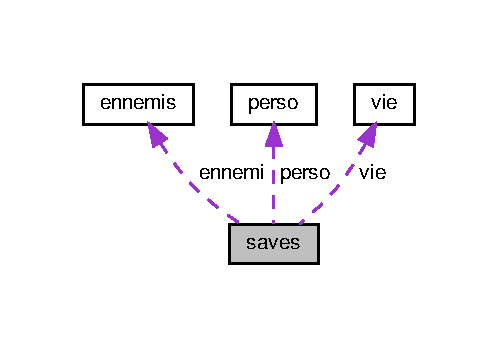
\includegraphics[width=239pt]{structsaves__coll__graph}
\end{center}
\end{figure}
\subsection*{Public Attributes}
\begin{DoxyCompactItemize}
\item 
\mbox{\Hypertarget{structsaves_a4ba3cba27704215b96311513ee206401}\label{structsaves_a4ba3cba27704215b96311513ee206401}} 
\hyperlink{structperso}{perso} {\bfseries perso}
\item 
\mbox{\Hypertarget{structsaves_a4797f7d3b3a1bf30019ec24e4f20b3f1}\label{structsaves_a4797f7d3b3a1bf30019ec24e4f20b3f1}} 
S\+D\+L\+\_\+\+Rect {\bfseries camera}
\item 
\mbox{\Hypertarget{structsaves_a94068fb387d61dec9a3f03296d5f2c38}\label{structsaves_a94068fb387d61dec9a3f03296d5f2c38}} 
\hyperlink{structennemis}{ennemis} {\bfseries ennemi}
\item 
\mbox{\Hypertarget{structsaves_ad07a79adf13feb4ffe0f035724ddb04b}\label{structsaves_ad07a79adf13feb4ffe0f035724ddb04b}} 
\hyperlink{structvie}{vie} {\bfseries vie}
\end{DoxyCompactItemize}


The documentation for this struct was generated from the following file\+:\begin{DoxyCompactItemize}
\item 
fonction.\+h\end{DoxyCompactItemize}

\hypertarget{structvie}{}\section{vie Struct Reference}
\label{structvie}\index{vie@{vie}}
\subsection*{Public Attributes}
\begin{DoxyCompactItemize}
\item 
\mbox{\Hypertarget{structvie_a02356445cb49a7290950ab15cebccdd9}\label{structvie_a02356445cb49a7290950ab15cebccdd9}} 
int {\bfseries nb}
\item 
\mbox{\Hypertarget{structvie_a916050892cf1e7b8039952dcafa44825}\label{structvie_a916050892cf1e7b8039952dcafa44825}} 
S\+D\+L\+\_\+\+Rect {\bfseries position}
\item 
\mbox{\Hypertarget{structvie_a564dc9c3b28da24d81318d703ebc4e59}\label{structvie_a564dc9c3b28da24d81318d703ebc4e59}} 
S\+D\+L\+\_\+\+Rect {\bfseries position2}
\item 
\mbox{\Hypertarget{structvie_a7616ae8ecc97b7fb2d92be6a858014ad}\label{structvie_a7616ae8ecc97b7fb2d92be6a858014ad}} 
S\+D\+L\+\_\+\+Surface $\ast$ {\bfseries fond1}
\item 
\mbox{\Hypertarget{structvie_a6ecad7f4161cb602faa27d2de9e3ee50}\label{structvie_a6ecad7f4161cb602faa27d2de9e3ee50}} 
S\+D\+L\+\_\+\+Surface $\ast$ {\bfseries fond2}
\item 
\mbox{\Hypertarget{structvie_a9763ef794bb12262f5826b911d20e42b}\label{structvie_a9763ef794bb12262f5826b911d20e42b}} 
S\+D\+L\+\_\+\+Surface $\ast$ {\bfseries fond3}
\item 
\mbox{\Hypertarget{structvie_a0b08072b8c7ec9e1adfd6e26b4fcb39f}\label{structvie_a0b08072b8c7ec9e1adfd6e26b4fcb39f}} 
S\+D\+L\+\_\+\+Surface $\ast$ {\bfseries fond4}
\item 
\mbox{\Hypertarget{structvie_adabeccdf7e33dd53ac6d85a24fc3931d}\label{structvie_adabeccdf7e33dd53ac6d85a24fc3931d}} 
S\+D\+L\+\_\+\+Surface $\ast$ {\bfseries fond5}
\end{DoxyCompactItemize}


The documentation for this struct was generated from the following file\+:\begin{DoxyCompactItemize}
\item 
playermov.\+h\end{DoxyCompactItemize}

\chapter{File Documentation}
\hypertarget{main_8c}{}\section{main.\+c File Reference}
\label{main_8c}\index{main.\+c@{main.\+c}}


Testing program  ragnarok.  


{\ttfamily \#include \char`\"{}fonction.\+h\char`\"{}}\newline
{\ttfamily \#include $<$unistd.\+h$>$}\newline
{\ttfamily \#include $<$S\+D\+L/\+S\+D\+L\+\_\+rotozoom.\+h$>$}\newline
{\ttfamily \#include $<$fcntl.\+h$>$}\newline
{\ttfamily \#include $<$termios.\+h$>$}\newline
Include dependency graph for main.\+c\+:
\nopagebreak
\begin{figure}[H]
\begin{center}
\leavevmode
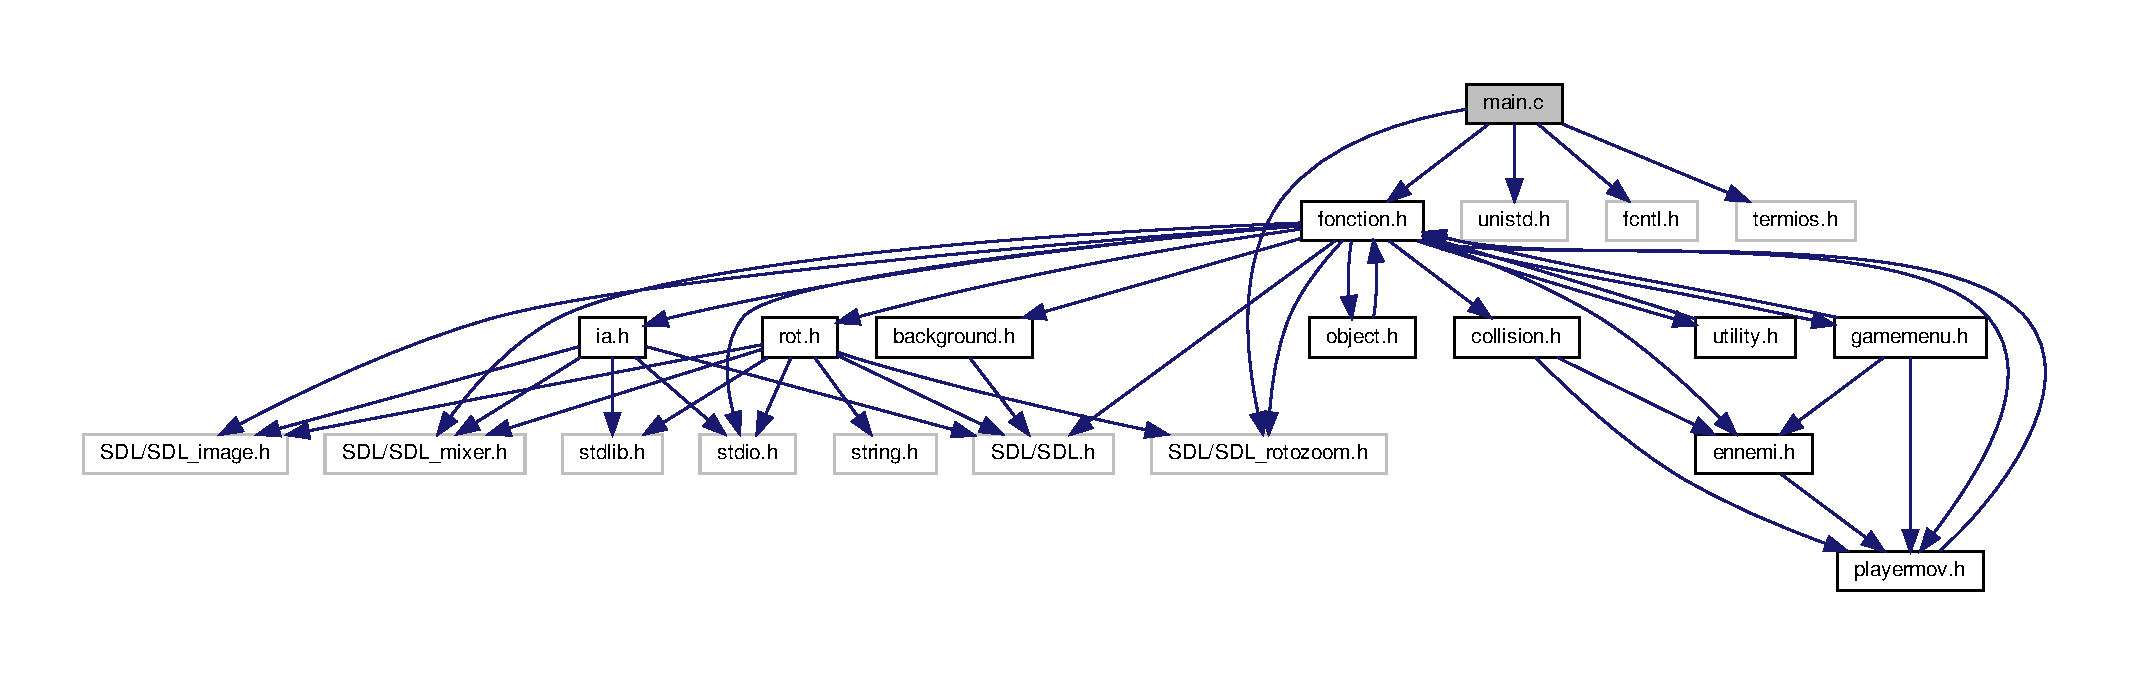
\includegraphics[width=350pt]{main_8c__incl}
\end{center}
\end{figure}
\subsection*{Functions}
\begin{DoxyCompactItemize}
\item 
\mbox{\Hypertarget{main_8c_ad15fd51e3a04ef8b8cc88202434480fb}\label{main_8c_ad15fd51e3a04ef8b8cc88202434480fb}} 
void {\bfseries savee} (\hyperlink{structennemis}{ennemis} ennemi, \hyperlink{structperso}{perso} \hyperlink{structperso}{perso}, \hyperlink{structvie}{vie} \hyperlink{structvie}{vie}, S\+D\+L\+\_\+\+Rect camera)
\item 
\mbox{\Hypertarget{main_8c_a443253fe2ba8b28fd860a78dc9ed1a8c}\label{main_8c_a443253fe2ba8b28fd860a78dc9ed1a8c}} 
void {\bfseries load} (\hyperlink{structennemis}{ennemis} $\ast$ennemi, \hyperlink{structperso}{perso} $\ast$\hyperlink{structperso}{perso}, \hyperlink{structvie}{vie} $\ast$\hyperlink{structvie}{vie}, S\+D\+L\+\_\+\+Rect $\ast$camera, int $\ast$continuer, int $\ast$save)
\item 
void \hyperlink{main_8c_a47dd868682e68ad2204e1a4054a2361d}{game} (S\+D\+L\+\_\+\+Surface $\ast$ecran, int save, int manette)
\begin{DoxyCompactList}\small\item\em void game \end{DoxyCompactList}\end{DoxyCompactItemize}


\subsection{Detailed Description}
Testing program  ragnarok. 

\begin{DoxyVersion}{Version}
0.\+1 
\end{DoxyVersion}
\begin{DoxyDate}{Date}
3/5/2019 Testing program for functionallity 
\end{DoxyDate}


\subsection{Function Documentation}
\mbox{\Hypertarget{main_8c_a47dd868682e68ad2204e1a4054a2361d}\label{main_8c_a47dd868682e68ad2204e1a4054a2361d}} 
\index{main.\+c@{main.\+c}!game@{game}}
\index{game@{game}!main.\+c@{main.\+c}}
\subsubsection{\texorpdfstring{game()}{game()}}
{\footnotesize\ttfamily void game (\begin{DoxyParamCaption}\item[{S\+D\+L\+\_\+\+Surface $\ast$}]{ecran,  }\item[{int}]{save,  }\item[{int}]{manette }\end{DoxyParamCaption})}



void game 


\begin{DoxyParams}{Parameters}
{\em ecran} & our screen of the game \\
\hline
{\em save} & to load our game \\
\hline
{\em manette} & to chose the play mode \\
\hline
\end{DoxyParams}
\begin{DoxyReturn}{Returns}
return nothing 
\end{DoxyReturn}

%--- End generated contents ---

% Index
\backmatter
\newpage
\phantomsection
\clearemptydoublepage
\addcontentsline{toc}{chapter}{Index}
\printindex

\end{document}
